\section{Introduction}
In this assignment I have to analyze for a financial institute data and make suggestions for the company. The event log is taken from the information system while it is running. 

All researches were done with ProM as ecpected from us. The data contains three types of activities (taken from the Assignment):

\begin{enumerate}
	\item Event names that start with "App\_" refer to status changes of applications. People make applications for a loan online.
	\item Event names that start with "P\_" refer to status changes of proposals, i.e. if the financial institute sees an opportunity to sell a loan to a customer, a proposal is sent to the customer.
	\item Events that start with "W\_" refer to activities performed by employees in the process, for example the call-center employees
\end{enumerate}

The data is analyzed in several steps to get a better idea of the process.

\section{General insights about the data set}

The given data set is generated between 1st Oct 2011 0:38:44 (Saturday) and 14th Mar 2012 16:04:54 (Wednesday) and contains 13087 cases with 262200 events executed. One case contains minimal 3 events and maximal 175. In average 20.035 events.

There are 4366 different variants of cases. There are 36 different events possible 
"W\_Complete\_Application + COMPLETE" (9.141\%), "W\_Complete\_Application + START" (8.967\%), "W\_Quotations + COMPLETE" (8.763\%), "W\_Quotations + START" (8.545\%), "App\_Fully\_Submission + COMPLETE" (4.991\%), "App\_Incomplete\_Submission + COMPLETE" (4.991\%), "W\_Handeling\_Incomplete\_Dossiers + COMPLETE" (4.35\%), "W\_Handeling\_Incomplete\_Dossiers + START" (4.348\%), "W\_Validation + COMPLETE" (3.011\%), "W\_Validation + START" (3.01\%), "App\_Rejection + COMPLETE" (2.912\%), "W\_Complete\_Application + SCHEDULE" (2.811\%), "App\_Pre\_Acceptation + COMPLETE" (2.81\%), "P\_Initiation + COMPLETE" (2.681\%), "P\_Selection + COMPLETE" (2.681\%), "P\_Sending + COMPLETE" (2.681\%), "W\_Quotations + SCHEDULE" (2.53\%), "W\_Handling\_Leads + COMPLETE" (2.249\%), "W\_Handling\_Leads + START" (2.249\%), "App\_Acceptation + COMPLETE" (1.95\%), "W\_Validation + SCHEDULE" (1.916\%), "App\_Finalization + COMPLETE" (1.913\%), "W\_Handling\_Leads + SCHEDULE" (1.82\%), "P\_Cancellation + COMPLETE" (1.394\%), "P\_Returning + COMPLETE" (1.317\%), "App\_Cancellation + COMPLETE" (1.071\%), "W\_Handeling\_Incomplete\_Dossiers + SCHEDULE" (0.909\%), "App\_Initiation + COMPLETE" (0.857\%), "App\_Approving + COMPLETE" (0.857\%), "App\_Registration + COMPLETE" (0.857\%), "P\_Acceptation + COMPLETE" (0.855\%), "P\_Rejection + COMPLETE" (0.306\%), "W\_Fraud\_Detection + COMPLETE" (0.103\%), "W\_Fraud\_Detection + START" (0.103\%), "W\_Fraud\_Detection + SCHEDULE" (0.047\%) and "W\_Changing\_Contact\_Details + SCHEDULE" (0.005\%).

The complete, start and shedule are more details about the state of the event. Just about the Workflow events we have more information about the state. 

All processes start in "App\_Fully\_Submission + COMPLETE" (100.0\%).

The processes can end in 13 different events:

"App\_Rejection + COMPLETE" (26.202\%), "W\_Validation + COMPLETE" (20.975\%), "W\_Handling\_Leads + COMPLETE" (17.07\%), "W\_Complete\_Application + COMPLETE" (14.816\%), "W\_Quotations + COMPLETE" (9.849\%), "App\_Cancellation + COMPLETE" (5.005\%), "W\_Handeling\_Incomplete\_Dossiers + COMPLETE" (3.454\%), "P\_Cancellation + COMPLETE" (2.132\%), "W\_Fraud\_Detection + COMPLETE" (0.436\%), "W\_Changing\_Contact\_Details + SCHEDULE" (0.031\%), "W\_Validation + START" (0.015\%), "App\_Registration + COMPLETE" (0.008\%) and "W\_Quotations + START" (0.008\%).

What you already see here, is that the process not always ended. All the process ending with a start event are probably not done now. This was to expected, because the data is picked during the running process.


\begin{figure}[!htbp]
\centering
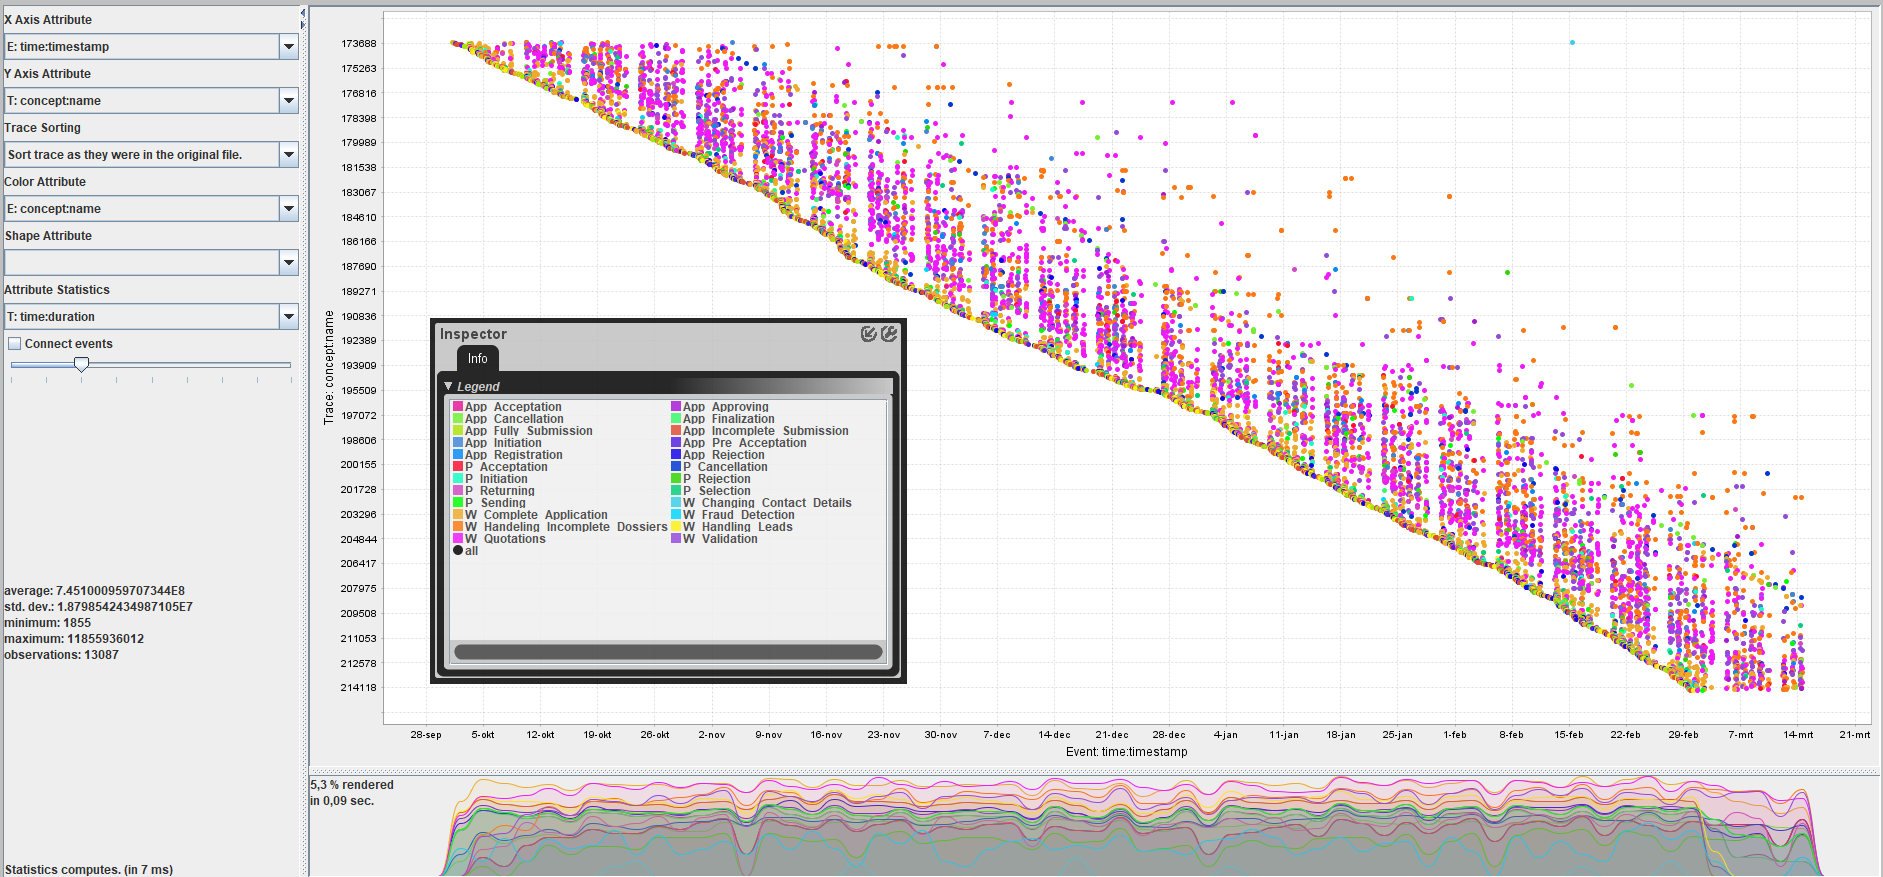
\includegraphics[width = 0.9\textwidth]{TotalDataDot.PNG}
\caption{Dotted chart of the data set}
\label{fig:WholeDat}
\end{figure}

Having a look at the whole data it can be seen, that there are just athe following events executes: "W\_Complete\_Application", "W\_Handling\_Leads", "App\_Incomplete\_Submission", "P\_Cancellation", "App\_Fully\_Submission" and "App\_Rejection". Furthermore is there a constant input of new cases. The events are mostly during the week executed same amount of times just "W\_Fraud\_Detection" and "W\_Changing\_Contact\_Details" have really deeps and ups. What is not surprising, because both are outlier behavior actions.